%%%%%%%%%%%%%%%%%%%%%%%%% NOTE %%%%%%%%%%%%%%%%%%%%%%%%%%%%
%% You can ignore everything from here until             %%
%% "Question 1: Introduction"                            %%
%%%%%%%%%%%%%%%%%%%%%%%%%%%%%%%%%%%%%%%%%%%%%%%%%%%%%%%%%%%
\documentclass[8pt]{article}
\usepackage{amsmath, amsfonts, amsthm, amssymb}  % Some math symbols
\usepackage{fullpage}
\usepackage{graphicx}
\usepackage[x11names, rgb]{xcolor}
\usepackage{graphicx}
\usepackage{tikz}
\usepackage{tcolorbox}
\usetikzlibrary{decorations,arrows,shapes}
\usepackage{float} % Add this package to control float placement
\usepackage{etoolbox}
\usepackage{enumerate}
\usepackage{listings}
\lstset{
    language=Python,           % Set the language of the code
    basicstyle=\footnotesize\ttfamily,
    keywordstyle=\color{blue}, % Set color for keywords
    commentstyle=\color{gray}, % Set color for comments
    stringstyle=\color{red},   % Set color for strings
    numbers=left,              % Display line numbers on the left
    numberstyle=\tiny\color{gray}, % Style for line numbers
    frame=single,              % Add a frame around the code
    breaklines=true            % Allow line breaking
}


\setlength{\parindent}{0pt}
\setlength{\parskip}{5pt plus 1pt}

\newcommand{\N}{\mathbb N}
\newcommand{\E}{\mathbb E}
\newcommand{\V}{Var}
\renewcommand{\P}{\mathbb P}
\newcommand{\f}{\frac}


\newcommand{\nopagenumbers}{
    \pagestyle{empty}
}

\def\indented#1{\list{}{}\item[]}
\let\indented=\endlist

\providetoggle{questionnumbers}
\settoggle{questionnumbers}{true}
\newcommand{\noquestionnumbers}{
    \settoggle{questionnumbers}{false}
}

\newcounter{questionCounter}
\newenvironment{question}[2][\arabic{questionCounter}]{%
    \addtocounter{questionCounter}{1}%
    \setcounter{partCounter}{0}%
    \vspace{.25in} \hrule \vspace{0.4em}%
        \noindent{\bf \iftoggle{questionnumbers}{#1: }{}#2}%
    \vspace{0.8em} \hrule \vspace{.10in}%
}{$ $\newpage}

\newcounter{partCounter}[questionCounter]
\renewenvironment{part}[1][\alph{partCounter}]{%
    \addtocounter{partCounter}{1}%
    \vspace{.10in}%
    \begin{indented}%
       {\bf (#1)} %
}{\end{indented}}

\def\show#1{\ifdefempty{#1}{}{#1\\}}

\newcommand{\header}{%
\begin{center}
    {\Large \show\myhwname}
    \show\myname
    \show\myemail
    \show\mysection
    \show\hwname
\end{center}}

\usepackage{hyperref} % for hyperlinks
\hypersetup{
    colorlinks=true,
    linkcolor=blue,
    filecolor=magenta,      
    urlcolor=blue,
}

%%%%%%%%%%%%%%%%% Identifying Information %%%%%%%%%%%%%%%%%
%% For 312, we'd rather you DIDN'T tell us who you are   %%
%% in your homework so that we're not biased when        %%
%% So, even if you fill this information in, it will not %%
%% show up in the document unless you uncomment \header  %%
%% below                                                 %%
%%%%%%%%%%%%%%%%%%%%%%%%%%%%%%%%%%%%%%%%%%%%%%%%%%%%%%%%%%%
\newcommand{\myhwname}{DS288 (AUG) 3:0 Numerical Methods }
\newcommand{\myname}{Naman Pesricha }
\newcommand{\myemail}{namanp@iisc.ac.in}
\newcommand{\hwname}{\textbf{Homework-3}}
\newcommand{\mysection}{SR - 24115}
%%%%%%%%%%%%%%%%%%%%%%%%%%%%%%%%%%%%%%%%%%%%%%%%%%%%%%%%%%%

%%%%%%%%%%%%%%%%%%% Document Options %%%%%%%%%%%%%%%%%%%%%%
\noquestionnumbers
\nopagenumbers
%%%%%%%%%%%%%%%%%%%%%%%%%%%%%%%%%%%%%%%%%%%%%%%%%%%%%%%%%%%

\begin{document}
\header

\begin{question} {Q1 Exercise Set 3.2, Problem \#12 in Text (Page-124). Be sure to read the note about inverse
interpolation directly above the problem. Solve this problem using an iterated interpolation approach (i.e., Neville’s algorithm). Report the relative error of your result and what value you used for the exact solution. [1.5 points]
}

\begin{table}[H]
\centering
\begin{tabular}{c c c c c c }
\hline
$i$ & $y = x - e^x$ & $ x = Q_{i0}$ & $Q_{i1}$ & $Q_{i2}$ & $Q_{i3}$ \\
\hline
0 & -0.440818 & 0.3 & -         & -         & - \\
1 & -0.270320 & 0.4 & 5.585473e-01 & -       & - \\
2 & -0.106531 & 0.5 & 5.650416e-01 & 5.671112e-01 & - \\
3 & 0.051188 & 0.6 & 5.675448e-01 & 5.671463e-01 & \textbf{5.671426e-01}\\
\hline
\end{tabular}
\caption{Inverse interpolation table using \textsc{nevilles}  for finding root of $x = f^{-1}(y)$. $Q_{ij}$ is the polynomial approximation that agrees with $[x_{i-j}, x_{i-j+1}, ... , x_{i} ].$}
\label{tab:data_table}
\end{table}

\begin{table}[H]
\centering
\begin{tabular}{c c c c c}
\hline
 $i$ & Relative Error $Q_{i,0}$ & Relative Error $Q_{i,1}$ & Relative Error $Q_{i,2}$ & Relative Error $Q_{i,3}$ \\
\hline
1 & 4.710331e-01 & - & - & - \\
2 & 2.947109e-01 & 1.515662e-02 & - & - \\
3 & 1.183886e-01 & 3.705734e-03 & 5.655048e-05 & - \\
    4 & 5.793370e-02 & 7.079698e-04 & 5.254266e-06 & \textbf{1.175861e-06} \\
\hline
\end{tabular}
\caption{Relative errors for the polynomials $Q_{ij}$ }
\label{tab:relative_errors}
\end{table}

\begin{center}
    Value used for exact solution (computed from \textsc{bisectionMethod}) \\
    \hfill \\
    \boxed{$$x^{*} = 0.5671432904$$} \\ 
    \hfill \\
    We get the least relative error in $Q_{43}$ \\
    \hfill \\
    \boxed{Computed Value = 5.671426e-01} \\
    \hfill \\
    \boxed{Relative Error ($$Q_{43}$$) = 1.175861e-06}
    
\end{center}

\hrule  
\end{question}

\begin{question}{Q2 In some applications one is faced with the problem of interpolating points which lie on
a curved path in the plane, for example in computer printing of enlarged letters. Often
the complex shapes (i.e., alphabet characters) cannot be represented as a function of x
because they are not single-valued. One approach is to use \textit{Parametric Interpolation.}
Assume that the points along a curve are numbered $P_1, P_2, ..., P_n$ as the curved path
is traversed and let $d_i$ be the (straight-line) distance between $P_i$ and $P_{i+1}$. Then define
$t_i = \Sigma^{i=1}_{j=1}dj$
, for for i =1, 2, ..., n (i.e.,$ t_1 = 0, t_2 = d_1, t_3 = d_1+d_2$, etc). If $P_i = (x_i
, y_i)$, one
can consider two sets of data ($t_i
, x_i$) and ($t_i
, y_i$) for i = 1, 2, ...n which can be interpolated
independently to generate the functions f(t) and g(t), respectively. Then $P(f(t), g(t))$
for $0 \leq t \leq t_n$ is a point in the plane and as t is increased from 0 to $t_n$, P(t) interpolates
the desired shaped (hopefully!). Interpolation of the data given below via this method
should produce a certain letter. Adapt your algorithm from problem (1) to perform the
interpolations on f(t) and g(t) where t is increased from 0.0 to 12.0 in steps of $dt$ (see
data below). Report the value of $dt$ you use to achieve ‘reasonable’ results. Turn in a
plot of your interpolated shape (not the numeric values of P(t)) as well as plots of f(t)
and g(t) individually. [3 points]}

For a very low value of dt(= 0.1250), we can visualize the value of $P(t)$, $f(t)$ and $g(t)$
\begin{figure}[H]
    \begin{minipage}{0.32\textwidth}
        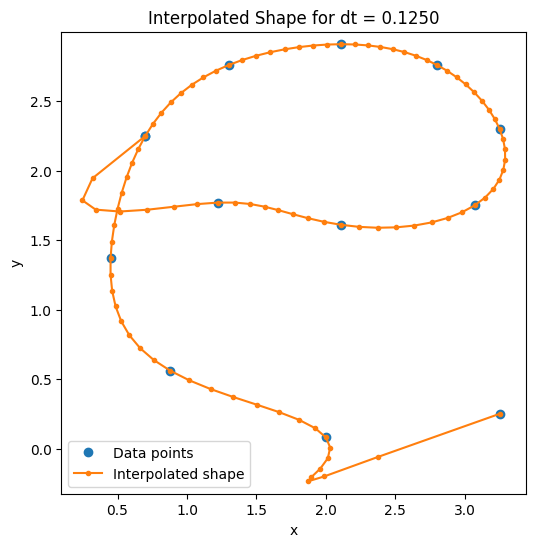
\includegraphics[width=\textwidth]{HW3/Q2images/e_0.1250.png} % Replace with your figure file
        \caption{$P(f(t), g(t))$ at dt = 0.125}
        \label{}
    \end{minipage}%
    \begin{minipage}{0.67\textwidth}

        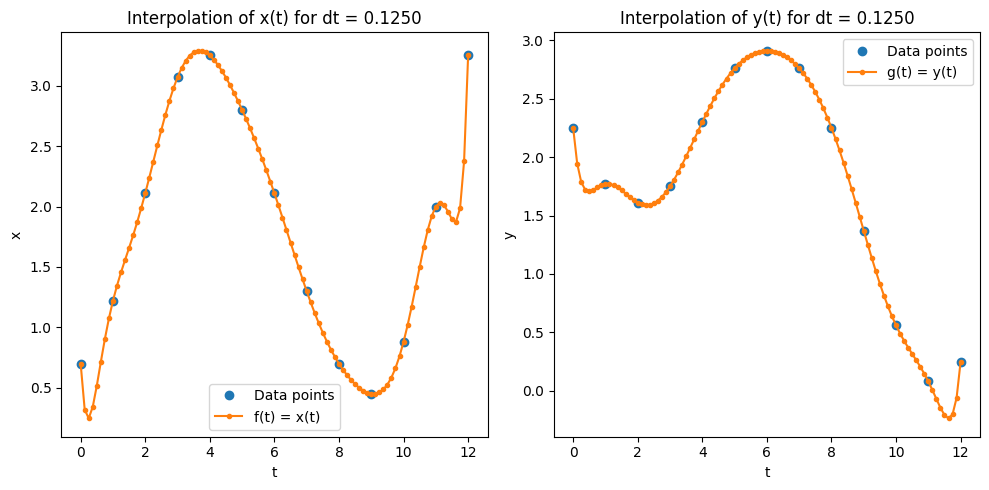
\includegraphics[width=\textwidth]{HW3/Q2images/xy_0.1250.png} % Replace with your figure file
        \caption{$x = f(t)$ and $y = g(t)$ for dt = 0.1250}
        \label{fig:fig2}
    \end{minipage}%
\end{figure}


\begin{center}
    This curve is smooth, but we can see the spurious (oscillations) at the end points. This is because the underlying polynomial of neville's algorithm is \textsc{lagrange} which is a \textit{Global Interpolating Polynomial} and hence the oscillations are observed. We can use a larger value of \\ 
    \hfill \\
    \boxed{$$dt = 0.8$$} \\
    \hfill \\
    to get a more reasonable curve which looks more like the letter \textbf{'e'} (but is not as smooth.) \\
    \hfill \\

    We can see that there's a clear tradeoff between number of smoothness ($\downarrow dt$) and avoiding oscillations at end points ($\uparrow dt$).
\end{center}

\begin{figure}[H]
    \begin{minipage}{0.32\textwidth}
        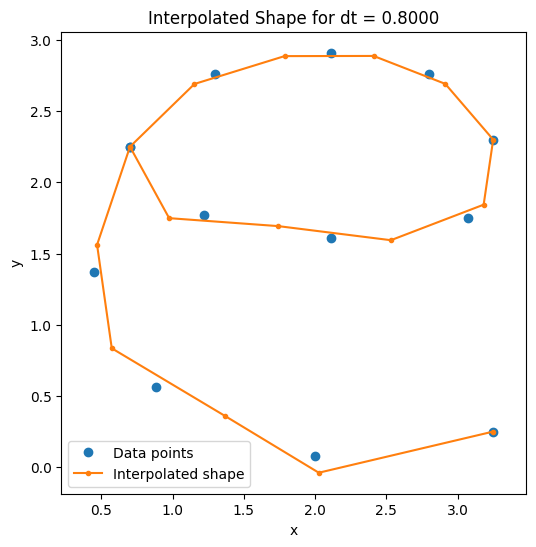
\includegraphics[width=\textwidth]{HW3/Q2images/e_0.8.png} % Replace with your figure file
        \caption{$P(f(t), g(t))$ at dt = 0.8}
        \label{}
    \end{minipage}%
    \begin{minipage}{0.67\textwidth}

        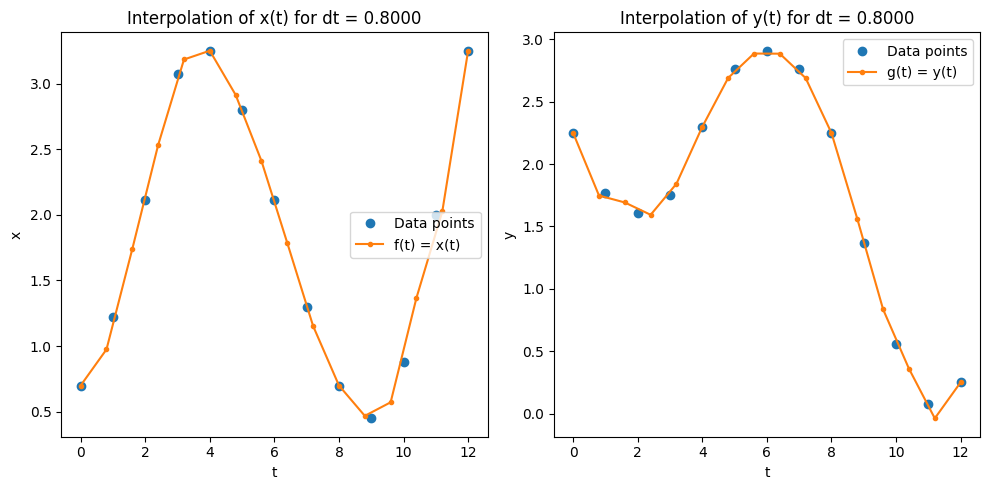
\includegraphics[width=\textwidth]{HW3/Q2images/xy_0.8.png} % Replace with your figure file
        \caption{$x = f(t)$ and $y = g(t)$ for dt = 0.1250}
    \end{minipage}%
\end{figure}

\hrule

\end{question}

\begin{question}{Q3 Repeat problem (2) with a natural cubic spline. Also report all four coefficients for each
of the cubics which comprise the interpolants for both f(t) and g(t). How does your letter
compare with that produced in problem (2)? Explain any differences. [3.5 points]
}

\begin{figure}[H]
    \begin{minipage}{0.32\textwidth}
        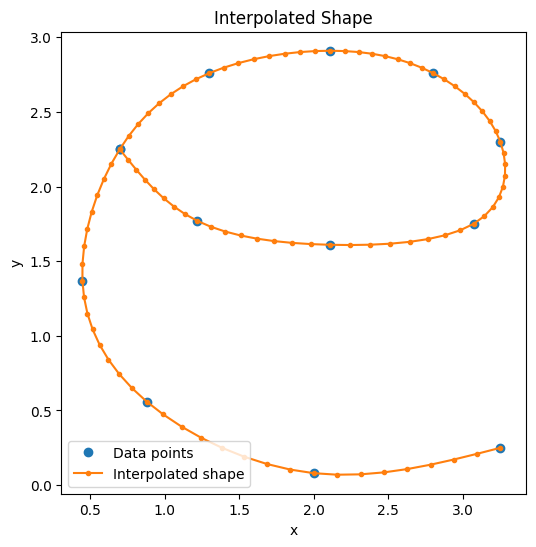
\includegraphics[width=\textwidth]{HW3/Q3images/e.png} % Replace with your figure file
        \caption{$P(t)$ for cubic spline.}
        \label{}
    \end{minipage}%
    \begin{minipage}{0.67\textwidth}

        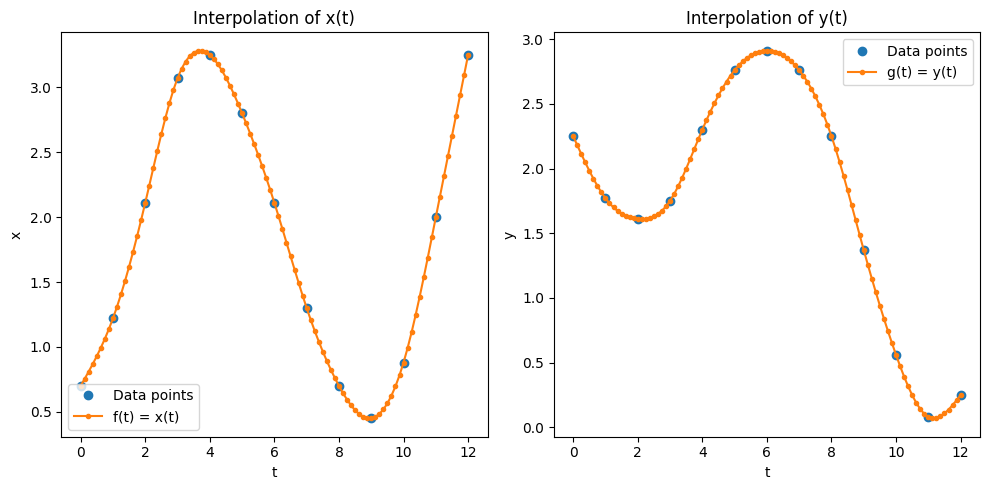
\includegraphics[width=\textwidth]{HW3/Q3images/xy.png} % Replace with your figure file
        \caption{$x = f(t)$ and $y = g(t)$ for dt=0.1250 for cubic spline}
        \label{fig:fig2}
    \end{minipage}%
\end{figure}

\begin{table}[H]
\centering
\begin{tabular}{c c c c c}
\hline
\textbf{Section} & \textbf{a} & \textbf{b} & \textbf{c} & \textbf{d} \\
\hline
0 & 8.2085e-02 & -1.1102e-16 & 4.3791e-01 & 7.0000e-01 \\
1 & -4.0427e-02 & 2.4626e-01 & 6.8417e-01 & 1.2200e+00 \\
2 & -2.2038e-01 & 1.2497e-01 & 1.0554e+00 & 2.1100e+00 \\
3 & 7.1935e-02 & -5.3616e-01 & 6.4422e-01 & 3.0700e+00 \\
4 & 8.2637e-02 & -3.2035e-01 & -2.1229e-01 & 3.2500e+00 \\
5 & -1.2481e-02 & -7.2441e-02 & -6.0508e-01 & 2.8000e+00 \\
6 & 8.7289e-02 & -1.0989e-01 & -7.8740e-01 & 2.1100e+00 \\
7 & -6.6750e-03 & 1.5198e-01 & -7.4531e-01 & 1.3000e+00 \\
8 & 7.9411e-02 & 1.3196e-01 & -4.6137e-01 & 7.0000e-01 \\
9 & 1.9031e-02 & 3.7019e-01 & 4.0779e-02 & 4.5000e-01 \\
10 & -1.4553e-01 & 4.2728e-01 & 8.3825e-01 & 8.8000e-01 \\
11 & 3.1069e-03 & -9.3207e-03 & 1.2562e+00 & 2.0000e+00 \\
\hline
\end{tabular}
\caption{Coefficients for $f(t)$ for equation $S_i = a_i(x-x_i)^3 + b_i(x-x_i)^2 + c_i(x-x_i) + d_i$}
\label{tab:oginal_matrix_transpose_with_section}
\end{table}

\tc

\begin{table}[H]
\centering
\begin{tabular}{c c c c c}
\hline
\textbf{Section} & \textbf{a} & \textbf{b} & \textbf{c} & \textbf{d} \\\hline
0 & 7.2213e-02 & 1.1102e-16 & -5.5221e-01 & 2.2500e+00 \\
1 & -4.1067e-02 & 2.1664e-01 & -3.3557e-01 & 1.7700e+00 \\
2 & 7.2053e-02 & 9.3440e-02 & -2.5493e-02 & 1.6100e+00 \\
3 & -1.3715e-01 & 3.0960e-01 & 3.7755e-01 & 1.7500e+00 \\
4 & -2.3466e-02 & -1.0184e-01 & 5.8531e-01 & 2.3000e+00 \\
5 & 1.1010e-02 & -1.7224e-01 & 3.1123e-01 & 2.7600e+00 \\
6 & -1.0574e-02 & -1.3921e-01 & -2.1795e-04 & 2.9100e+00 \\
7 & -2.8714e-02 & -1.7093e-01 & -3.1036e-01 & 2.7600e+00 \\
8 & 1.1543e-01 & -2.5707e-01 & -7.3836e-01 & 2.2500e+00 \\
9 & 6.9979e-03 & 8.9216e-02 & -9.0621e-01 & 1.3700e+00 \\
10 & 1.1658e-01 & 1.1021e-01 & -7.0679e-01 & 5.6000e-01 \\
11 & -1.5332e-01 & 4.5995e-01 & -1.3663e-01 & 8.0000e-02 \\
\hline
\end{tabular}
\caption{Coefficients for $g(t)$ for equation $S_j = a_j(y-y_i)^3 + b_j(y-y_j)^2 + c_j(y-y_j) + d_j$}
\label{tab:new_matrix_transpose_with_section}
\end{table}




    
\end{question}

\begin{question}{Q4 Consider the oscillograph record of the free-damped vibrations of a structure. From
vibration theory, it is known that for viscous damping (damping proportional to velocity) the envelop of such a vibration (i.e., the curve through the peaks of the oscillations) is an
exponential function of the form 

$$ y = be^{-2\pi a x}$$

where x is the cycle number, y is the corresponding amplitude and a is a damping factor.
Using the three data points shown in the figure, determine a and b that result from a best
fit based on the least-squares criterion. Use a linear least squares approach by suitable
change of variable. You may solve this problem “by hand” if you wish. \\
An alternate approach to this problem would be to construct a nonlinear least-squares
fit using the data directly as given. Would this approach lead to exactly the same a and
b values you determine above (assuming perfect math, i.e., no rounding errors in either
case)?. [2 points]}
\begin{table}[H]
\centering
\begin{tabular}{c c c c}
\hline
\textbf{Name} & \textbf{Prediction} & \textbf{Error} \\
\hline
Transformed approach & $pred_{transformed}$ & $E_{transformed}(y_i, \hat{y_i})$ = $\sum [\log(y_i) - \log\hat{(y_i)}]^2$\\
 Non-Linear least squares  & $pred_{non-linear}$ & $E_{non-linear}(y_i, \hat{y_i}) = \sum [(y_i) - \hat{(y_i)}]^2 $ \\
\hline
\end{tabular}
\caption{Terminologies used in answer 4.}
\label{tab:your_label_here}
\end{table} 

\begin{center}
    By using the \textbf{Transformed approach}, we can transform the problem to a linear problem by taking $log$ on both sides.
    {$$ y = be^{-2\pi a x} \equiv \log{y} = \log{b} - 2 \pi a x$$} \\
    Solving this linear equation using linear least squares we get. \\
    \hfill \\
    \boxed{$$a_{transformed} = 0.00609$$}  \boxed{$$b_{transformed} = 16.86397$$ } \\
    \hfill \\
    Using the \textbf{Non-linear approach},  we get the following values of coefficients:\\
    \hfill \\
    \boxed{$$a_{non-linear} = 0.00618$$}  \boxed{$$b_{non-linear} = 16.96953$$ } \\
    \hfill \\
    \begin{tcolorbox}
        We will get \textbf{different} a and b values using the \textbf{non-linear approach} (assuming perfect maths) as both approaches are minimizing different error functions $E_{transformed}$ and $E_{non-linear}$. From the table below, we can see that the $pred_{non-linear}$ minimizes $E_{non-linear}$ and $pred_{transformed}$ minimizes $E_{transformed}$. Moreover, the \textbf{transformed} approach is not the least squares approximation of the original problem.
    \end{tcolorbox}

    $pred_{transformed}$ = [ 16.8639, 9.14577, 4.95999 ] ,  $pred_{non-linear}$ = [ 16.9695, 9.11345, 4.89436 ]
    
    \begin{table}[H]
        \centering
        \begin{tabular}{c c c}
            \hline
             \textbf{Approach} & $pred_{tarnsformed}$& $pred_{non-linear}$ \\
             \hline
              $E_{transformed}(y_i, \hat{y_i})$ & \textbf{0.000387} & 0.000616\\
              $E_{non-linear}(y_i, \hat{y_i})$ & 0.041354  & \textbf{0.024959}\\
            \hline
        \end{tabular}
        \caption{$pred_{non-linear}$ minimizes $E_{non-linear}$ and $pred_{transformed}$ minimizes $E_{transformed}$.}
        \label{tab:my_label}
    \end{table}
    \hrule

\end{center}

\end{question}

\end{document}



